\section{CCAT Class}
\label{Section:ComputerControlledAutomaticTransmission}
The \emph{ComputerControlledAutomaticTransmission} class is formalized thanks to the code reported in Listing~\ref{Code:ComputerControlledAutomaticTransmission} while Figure~\ref{Figure:CCAT} shows the \emph{big picture} of our complete designed.

\lstinputlisting[language=TRIO,tabsize=4,numbers=left,numberstyle=\small,basicstyle=\small,breaklines,breakatwhitespace,frame=single,caption=ComputerControlledAutomaticTransmission.trio,label=Code:ComputerControlledAutomaticTransmission]{../trio/ComputerControlledAutomaticTransmission.trio}

\thispagestyle{empty}
\begin{figure}[!p]
\vspace{-3 cm}
\centerline{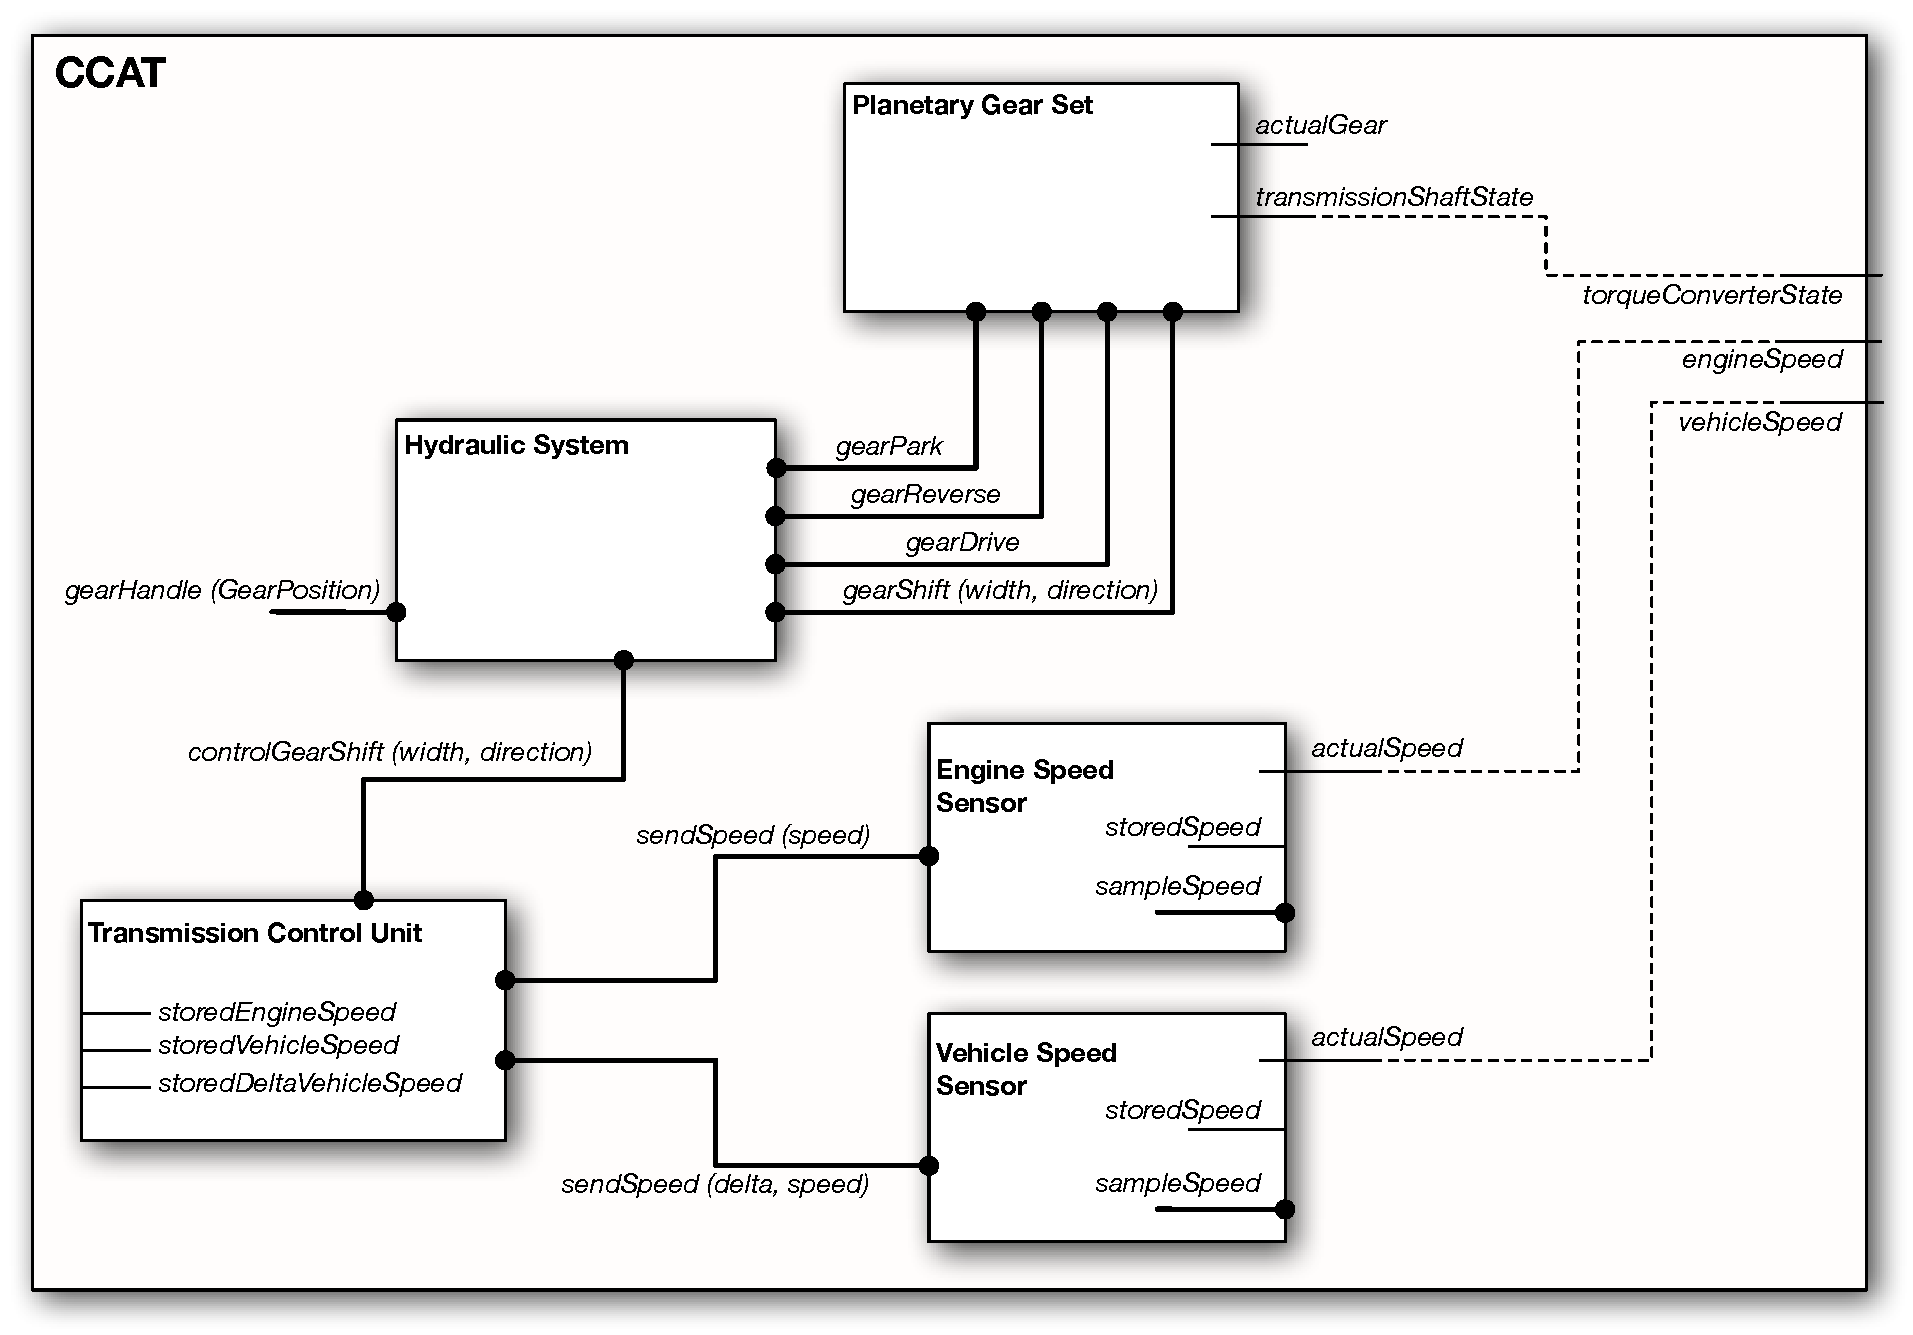
\includegraphics[scale=0.8,angle=-90]{images/CCAT.pdf}}
\caption{Computer Controller Automatic Transmission}
\label{Figure:CCAT}
\end{figure}

\newpage
Due to the fact that a TRIO specification is not decidable we have decided to focus our verification process only on the Hydraulic System, described in Section~\ref{Section:HydraulicSystem}, and on the Planetary Gear Set, described in Section~\ref{Section:PlanetaryGearSet} and we have used a decidable subset of the TRIO language.

The specification is reported in Listing~\ref{Code:ComputerControlledAutomaticTransmission2}.

\lstinputlisting[language=TRIO,tabsize=4,numbers=left,numberstyle=\small,basicstyle=\small,breaklines,breakatwhitespace,frame=single,caption=ComputerControlledAutomaticTransmission.trio,label=Code:ComputerControlledAutomaticTransmission2]{../t2p/ComputerControlledAutomaticTransmission.trio}

The same specification reported in Listings~\ref{Code:ComputerControlledAutomaticTransmission2} has been ported also in Zot and is listed in Listings~\ref{Code:ComputerControlledAutomaticTransmission3}.

\lstinputlisting[language=Zot,tabsize=4,numbers=left,numberstyle=\small,basicstyle=\small,breaklines,breakatwhitespace,frame=single,caption=ComputerControlledAutomaticTransmission.lisp,label=Code:ComputerControlledAutomaticTransmission3]{../zot/ComputerControlledAutomaticTransmission.lisp}
